\documentclass[10pt,conference]{IEEEtran}
% If the IEEEtran.cls has not been installed into the LaTeX system files,
% manually specify the path to it:
% \documentclass[conference]{../sty/IEEEtran}
\usepackage{graphicx}
\usepackage{subcaption}
\begin{document}

% paper title
\title{Identification of black hole states using matrix based methods: Timeseries analysis of RXTE satellite data}


% author names and affiliations
% use a multiple column layout for up to three different
% affiliations
%\author{
%\authorblockN{A. Chockalingam}
%\authorblockA{Dept.\ of Electrical Communication Engg.\\
%Indian Institute of Science \\
%Bangalore, 560012, India\\
%Email: spcom2016@gmail.com} \and
%\authorblockN{Rahul Vaze}
%\authorblockA{School of Technology and Computer Science\\
%Tata Institute of Fundamental Research\\
%Mumbai, 400005, India\\
%Email: spcom2016@gmail.com}
%\and
%\authorblockN{Animesh Kumar}
%\authorblockA{Dept.\ of Electrical Engg.\\
%Indian Institute of Technolgy \\
%Bombay, 400076, Mumbai India\\
%Email: spcom2016@gmail.com} 
%%\and
%%\authorblockN{Robert Calderbank}
%%\authorblockA{Department of Electrical Engineering\\
%%Princeton University \\
%%Princeton, NJ 08544, USA\\
%%Email: calderbk@math.princeton.edu} \and
%%\authorblockN{Habong Chung}
%%\authorblockA{Department of Electronic\\
%%\& Electrical Engineering\\
%%Hongik University\\
%%Seoul, Korea\\
%%Email: habchung@hongik.ac.kr}
%}
% avoiding spaces at the end of the author lines is not a problem with
% conference papers because we don't use \thanks or \IEEEmembership
% for over three affiliations, or if they all won't fit within the width
% of the page, use this alternative format:
% make the title area
\maketitle

\begin{abstract}
Black hole is one of the fascinating,  however mysterious, astrophysical  objects. In order to identify it one has to look at its environment, often forming a disc-like structure. This disc, called accretion disc, evolves with time transiting from one state to another. For example, in one extreme regime it shows temperature dependent radiations making the disc geometrically thin, and in yet another extreme  regime of time span however radiation turns out to be temperature independent making the disc hot and geometrically thick.  Nevertheless, in general, accretion disc lies in  states intermediate between the two extremes. The present mission is to capture black hole states  explicitly using PCA and SVD based decompositions. In order to do that we rely on timeseries data of black hole \textit{GRS 1915 + 105} obtained from RXTE satellite. As a black hole cannot be seen directly, identifying its states accurately could help in characterizing its properties. Earlier timeseries  analysis based on correlation integral approaches, supplemented by theory, argued for four specific states. However there are caveats when data themselves are not free from noise and the  appropriate method for such an analysis itself is exploratory. Present interdisciplinary study aims at, on one hand,  to cross-verify the previous inference, on the other hand to identify, if any,  novel characteristics of black holes. This is expected to have long standing implications in astrophysics and otherwise.
\end{abstract}

\section{Introduction}
One of the challenging problems in astrophysics is the understanding of black holes. As the black holes can not be seen directly, to identify it one has to look for its environment forming a disc like structure by the infalling matter called accretion disc. In this work, we focus on the black hole source GRS 1915+105, which presents several intriguing facets. One of the fundamental aspects of the understanding is to determine if the black hole source is a stochastic system or a non-stochastic one. The latter one is related to the well-known turbulent nature of the system. There are several studies that utilize the Correlation Integral (CI) approach to determine the characterization of the black hole data \cite{Mukhopadhyay2004, misra2006}. However, there can also be other approaches to understanding the same data by applying, for e.g.,  matrix-based methods such as Principal Component Analysis (PCA) and Singular Value Decomposition (SVD). It is useful to compare the inferences obtained using these two distinct approaches; the implications of the (dis)similarities in inferences, if any, could lead to questions about understanding the temporal dynamics of the system.

Interestingly, to quantify the properties of a black hole source, along with temporal features one has to look for spectral features as well, they together lead to the true nature of the source. If the source radiation is temperature dependent, it produces more like a blackbody radiation, namely multicolour blackbody or diskbb \cite{Shakura1973}. On the other hand, the temperature independent radiation consists of a power-law tail, named as PL \cite{chakrabarti1995,narayan1994}.
While the former leads the underlying accretion disc around the black hole to be geometrically thin, the latter leads to a geometrically thick disc.


Following are the major contributions of this paper:
\begin{itemize}
  \item We use PCA, an approach widely used for decorrelating features and dimensionality reduction, for characterizing a timeseries as stochastic vs non-stochastic. We propose a novel approach by iteratively computing eigenvalue ratios  of covariance matrix for different subintervals of the timeseries. We  derive multiple features from the eigenvalue ratios and use them to characterize the timeseries. Utility of the proposed approach is illustrated by comparing the results with previously established methods.
  \item We use SVD decomposition of the data matrix for identifying the temporal dynamics of the timeseries. A plot involving top two right singular vectors of the data matrix shows a clear distinction between stochastic and non-stochastic timeseries.
\end{itemize}
\section{Related Work}
Several groups have worked on distinguishing between stochastic and non-stochastic timeseries. The idea of utilizing Permutation Entropy (PE) to determine the complexity measure of a timeseries is explored in \cite{Bandt2002}. In the work reported in \cite{Boaretto2021}, a Neural Network based approach is used. A Neural Network is trained with noise to learn the parametrization of stochastic signals. The paper explores the idea of utilizing PE of a timeseries to determine if it is strongly correlated with known stochastic signals (noise).   The claim is that for non-stochastic signals the deviation of the parameter is relatively large as compared to that of the parameter of a stochastic signal.  Yet another approach has been to utilize graph theoretical tools. In the work reported in \cite{lacasa2010}, the authors have utilized the horizontal visibility algorithm in order to distinguish between stochastic and non-stochastic processes.

In the approach outlined in \cite{Brunton2016}, the authors combine the idea of sparsity and machine learning with non-linear dynamical systems, in order to determine the governing dynamics. Sparse regression is used to determine the fewest terms in the equations that govern the dynamics of the phenomenon. The user-defined dictionary of basis functions consists of well-known functions such as polynomials, trigonometric functions and exponentials. The coefficients corresponding to very few of these basis functions will be non-zero for a non-stochastic system. However, the optimal choice of dictionary for a specific choice of problem remains a challenge.

In this work we propose to utilize matrix based methods which do not require any assumptions about the underlying phenomenon.

\begin{figure*}[ht]
  \centering
  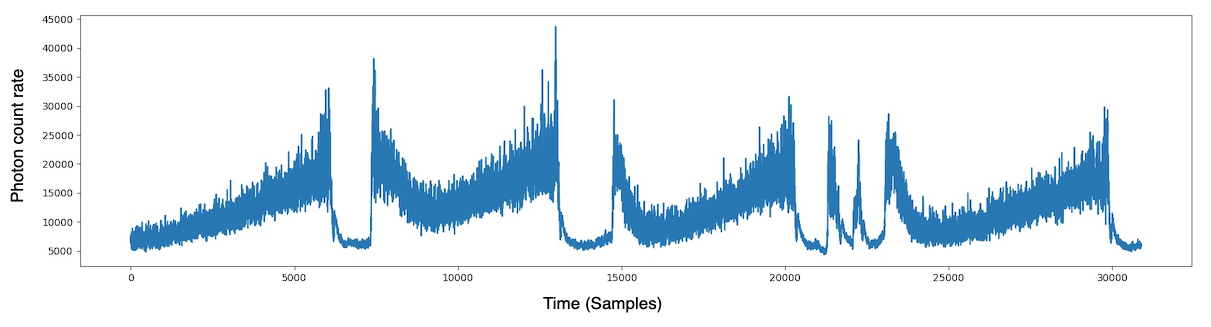
\includegraphics[width=0.8\linewidth]{theta_ts_edited.drawio.png}
  \caption{A representative non-stochastic timeseries of class $\theta$ of \textit{GRS 1915 + 105}. }
  \label{theta_ts}
\end{figure*}
\begin{figure*}[ht]
  \centering
  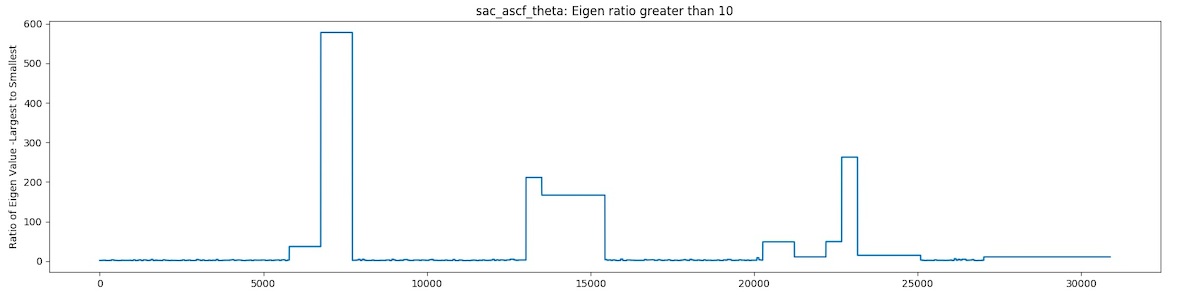
\includegraphics[width=0.8\linewidth]{theta_ts_eig.png}
  \caption{Plot of eigen-ratio of the  non-stochastic timeseries shown in Figure \ref{theta_ts}. }
  \label{theta_eig}
\end{figure*}

\section{Proposed Method}
In this work, we use two different matrix based approaches, one using PCA and the second using SVD, to characterize timeseries as stochastic vs non-stochastic.

\subsection{PCA Based approach}
In this approach, we utilize PCA to understand if the available data posseses a dominant orientation. This can be computed by splitting the timeseries into two halves, and computing the covariance matrix of these observations. The eigenvalues of this $2 \times 2$ covariance matrix will show one of the signatures: If the data indeed show any dominant direction (as in non-stochastic timeseries), then the larger eigenvalue will be significantly greater than the other. This will lead to a large ratio of the eigenvalues. On the other hand, if the data do not show any dominant direction (as in stochastic timeseries), then the two eigenvalues of the covariance matrix will be comparable. This will lead to small values of eigenvalue ratio.

Consider a timeseries consisting of $n$ values  $z_1, z_2 \mathellipsis z_n$. We begin by computing the eigenvalue ratio for the entire series using the following steps:
\begin{itemize}
  \item  Split the series into two halves $(z_1, z_2 \mathellipsis z_{\frac{n}{2}})$ and $(z_{\frac{n}{2} + 1}, \mathellipsis z_n)$.
  \item Compute covariance matrix, $C$,  by treating the samples in two halves as $n/2$ observations of two dimensional vectors.
  \item Compute eigenvalues, $\lambda_1$ and $\lambda_2$ of $C$,  and the eigenvalue ratio is computed as  $\lambda_1/\lambda_2$ where $\lambda_1 \ > \lambda_2$ (Eigenvalues of a covariance matrix are real).
\end{itemize}
If eigenvalue ratio for an interval is less than a predefined threshold (empirically determined as 10 for the given dataset), the interval is split into two subintervals of equal size and eigenvalue ratio for each sub-interval is computed. The process is repeated as long as the length of the sub-interval is greater than a predefined number of samples.

Using PCA analysis we have derived the following three features for each timeseries:
\begin{itemize}
  \item Maximum eigenvalue ratio (MER): This is the maximum value obtained as the ratio of the two eigenvalues of the covariance matrix of any sub-interval of the timeseries.
  \item Variance of eigenvalue ratio (VAR): This is the variance of the eigenvalue ratios of covariance matrices across sub-interval in the entire timeseries.
  \item Area under the eigenvalue ratio curve (Area): This measure captures the area under the curve of the eigenvalue ratio for the entire timeseries.
\end{itemize}


\subsection{SVD based approach}
In this approach, we form uncorrelated observation vectors from the raw timeseries data by utilizing the optimal value of embedding dimension \cite{misra2006}. A data matrix, $D$, is formed with each row  as the  time shifted version of the original timeseries. The time shift is chosen to be large enough so that each row can be viewed as a different observation vector of the same phenomenon. The temporal dynamics is understood by utilizing the right singular vectors of the SVD decomposition of the data matrix as given in equation (\ref{eqn:svd}). Columns of $U$ and $V$  form the left and right singular vectors respectively and $\Sigma$ is a block diagonal matrix with diagonal elements as the singular values, given by
\begin{equation}
  D = U \Sigma V^T.
  \label{eqn:svd}
\end{equation}
   We observe the plot of the top two right singular vectors (E1 and E2). For non-stochastic timeseries this plot is expected to show a specific patterned behavior (attractor behavior, where the plot follows a trajectory leaving a well-defined gap). On the other hand for stochastic timeseries, this behavior is absent.

\section{Results and Discussions}


\begin{figure*}[ht]
  \centering
  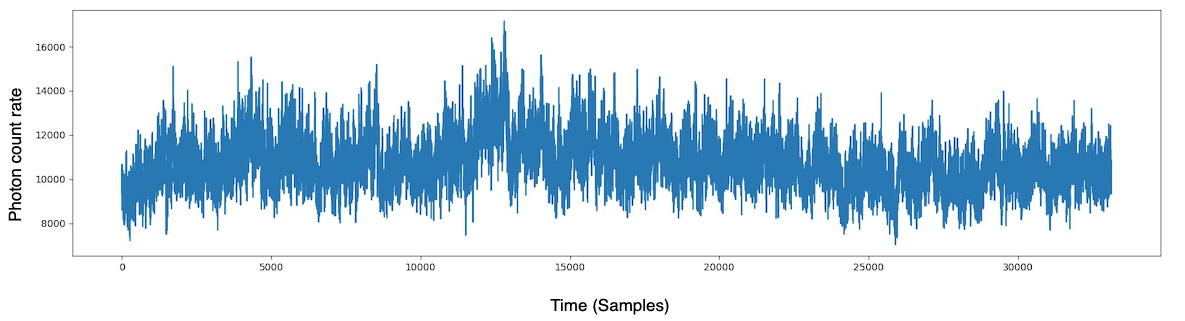
\includegraphics[width=0.9\linewidth]{phi_ts_edited.drawio.png}
  \caption{A representative stochastic timeseries of class $\phi$ of \textit{GRS 1915 + 105} }
  \label{phi_ts}
  \end{figure*}

\begin{figure*}[ht]
  \centering
  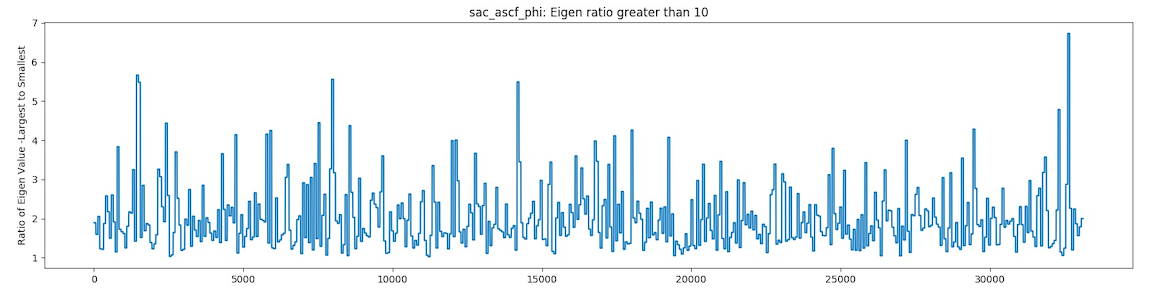
\includegraphics[width=0.9\linewidth]{phi_ts_eig.png}
  \caption{Plot of eigen-ratio of the stochastic timeseries shown in Figure \ref{phi_ts}.}
  \label{phi_eig}
\end{figure*}

\subsection{Results of PCA based analysis}

Figures \ref{theta_eig}  and \ref{phi_eig} show the eigenvalue ratio plots for non-stochastic and stochastic timeseries respectively. In our experiments using timeseries of 12 different classes of \textit{GRS 1915 + 105}, we compute the three PCA based features which are MER, VAR and Area. Table \ref{tab:results} lists the following quantities as described below:

\begin{enumerate}
  \item Column 1 gives the class of the timeseries \cite{Adegoke2018}.
  \item Column 2 gives the inference about the state of the timeseries using CI approach \cite{Adegoke2018}.
  \item Columns 3 and 4 give quantities Diskbb and  PL, respectively, which indicate the state of the black hole \cite{Adegoke2018}.
  \item The computed PCA based features: MER, VAR and Area  are tabulated in columns 5, 6 and 7 respectively.
\end{enumerate}

We have examined various clusters formed using above PCA features and have come up with the following guidelines in order to infer the state of black hole. For example a sample visualization of the clusters formed in the VAR-Area feature space is shown in Figure \ref{fig:variance_area_fs}.

\begin{itemize}
  \item MER: For stochastic timeseries, eigenvalue ratios  are small across the entire timeseries, typically lying in the range 1-20. This implies that MER  will also be small. On the other hand, for  non-stochastic timeseries the eigenvalue ratios are significantly high, typically reaching a few thousands in certain sub-intervals. Hence the MER for a non-stochastic timeseries is typically large.
  \item VAR: For a stochastic signal since the range of eigenvalue ratios is typically small, the VAR is also small. On the other hand, for a non-stochastic signal, since the eigenvalue ratios occupy a large range of values, VAR is typically high.
  \item Area: For a stochastic timeseries, since the eigenvalue ratios  are small the Area is also small. However, for a non-stochastic signal the eigenvalue ratios remain high for longer time intervals. Hence the Area is significantly higher.
\end{itemize}

Our inference using these PCA features are given in column 8 and finally the last column gives if there is a match between PCA based inference and CI based inference.

\begin{table*}[t]
\caption{Timeseries: Comparison between CI based label vs inference using proposed PCA features. The mismatched timeseries class, $\delta$, is shown in bold. (LC stands for Limit Cycle \cite{Adegoke2018} which is non-stochasitic.)}
\begin{center}
%\begin{tabular}{|c|c|c|c|c|c|c|c|c|c|c|}
  \begin{tabular}{|p{0.5cm}|p{1cm}|p{0.75cm}|p{0.5cm}|p{0.75cm}|p{1cm}|p{0.5cm}|p{1.8cm}|p{2.5cm}|p{3cm}|p{0.75cm}|}
\hline
Class & CI \newline Behavior & Diskbb & PL & MER & Variance & Area & Inference \newline PCA Features & SVD \newline Topological Features & Inference \newline SVD Topological features & Match \\
\hline
$\beta$ & F & 46 & 52 & 214 & 483 & 43 & Non-stochastic & &&Yes\\
\hline
$\theta$ & F & 11 &  88 & 577 & 778 & 58&Non-stochastic & &&Yes \\
\hline
$\lambda$ & F & 54 & 46 & 600 & 6782 & 314 & Non-stochastic & &Non-stochastic&Yes \\
\hline
$\kappa$ & F & 59 & 51 & 700 & 5199 & 144 & Non-stochastic & &Non-stochastic&Yes \\
\hline
$\mu$ & F & 56 & 41 & 50 & 51 & 12 & Non-stochastic & &Non-stochastic&Yes \\
\hline
$\nu$ & F & 28 & 72 & 30 & 32 & 16 & Non-stochastic & &Non-stochastic&Yes\\
\hline
$\alpha$ & F & 23 & 77 & 30 & 1.9 & 27.7 & Non-stochastic & &Non-stochastic&Yes \\
\hline
$\rho$ & LC & 28 & 72 & 60 & 147 & 35 & Non-stochastic & &Non-stochastic&Yes \\
\hline
\textbf{$\delta$} & \textbf{S} & \textbf{48} & \textbf{50} & \textbf{42} & \textbf{9.74} & \textbf{26.2} & \textbf{Non-stochastic} &&& \textbf{No} \\
\hline
$\phi$ & S & 50 & 34 & 7 & 0.5 & 15 & Stochastic &&Stochastic& Yes \\
\hline
$\gamma$ & S & 60 & 31 & 12 & 1 & 16 & stochastic &&Stochastic& Yes \\
\hline
$\chi$ & S & 09 & 89 & 5.6 & 0.25 & 6.05 & Stochastic &&Stochastic& Yes \\
\hline
\end{tabular}
\label{tab:results}
\end{center}
\end{table*}

\begin{figure}
    \centering
    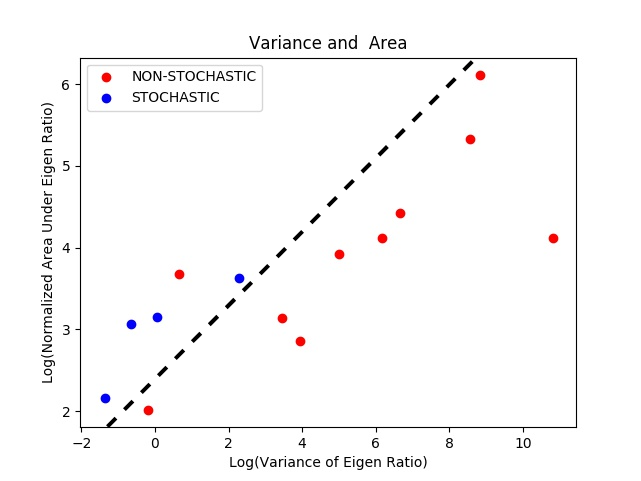
\includegraphics[width=.9\linewidth]{var_area_fs.drawio.png}
    \caption{Feature space (VAR and Area) shows that the two classes are well separated. The dashed line shows the decision boundary separating the two classes. The label of one of the timeseries is ambiguous.}
    \label{fig:variance_area_fs}
\end{figure}

We observe that the PCA based features, VAR and Area, result in visible clustering as shown in Figure \ref{fig:variance_area_fs}. This could be attributed to the fact that   these features take into account the entire span of timeseries and hence form robust feature space. Our inference for each of the timeseries using above guidelines is shown in column 8 of Table \ref{tab:results}. It is noticed that our inference matches with the analysis result based on CI in all the cases except for class $\delta$. According to the CI analysis $\delta$ turns out to be in between classes Slim disc and General Advective Accretion Flow (GAAF) \cite{Adegoke2018}. However, the present analysis shows that $\delta$ falls in between Advection Dominated Accretion Flow (ADAF) and Keplerian disc, as explained in \cite{Adegoke2018}.


\subsection{Results of SVD based analysis}

\begin{figure}[ht]
  \centering
  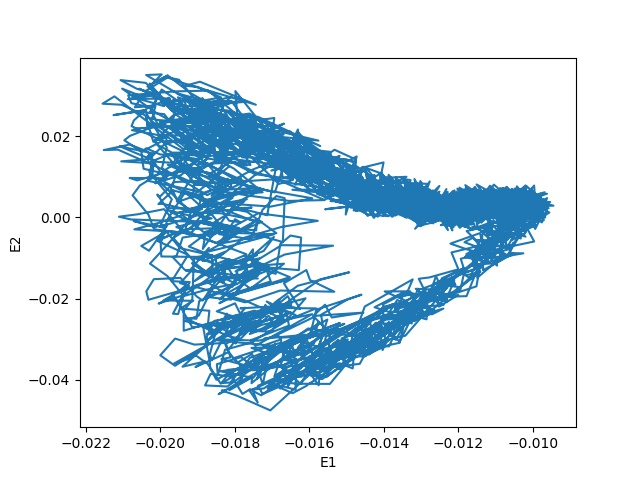
\includegraphics[width=\linewidth]{rho_svd.jpg}
  \caption{Plot of E1 Vs E2 (top two right singular vectors) of data matrix for  timeseries $\rho$ (non-stochastic) of \textit{GRS 1915 + 105}.}
  \label{svd_rho}
\end{figure}

From SVD decomposition of the data matrix, we pick up the top 2 right singular vectors (E1, E2) corresponding to the temporal dynamics and plot E1 vs E2 for each timeseries. Figure \ref{svd_rho} shows the E1-E2 plot for timeseries $\rho$ which is of type Limit Cycle \cite{misra2006} (non-stochastic). The expected attractive behavior is clearly visible in the plot. Figures \ref{chi_svd} and \ref{lamda_svd} show the plots for class $\chi$ and $\lambda$  which  according to CI approach , are stochastic and non-stochastic respectively. From the plots  using SVD based analysis also, it is clear  that the timeseries depicted in Figure \ref{chi_svd} is stochastic, while the timeseries depicted in Figure \ref{lamda_svd} is non-stochastic.

\begin{figure}[ht]
  \centering
  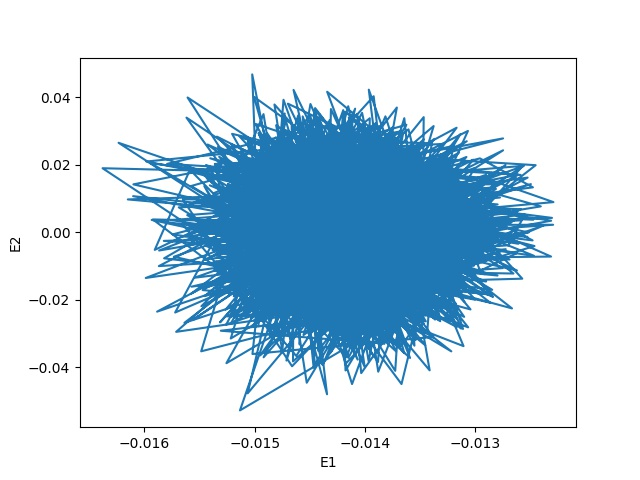
\includegraphics[width=\linewidth]{chi_svd.jpg}
  \caption{Plot of E1 Vs E2 (top two right singular vectors) of data matrix for  timeseries $\chi$ (stochastic) of \textit{GRS 1915 + 105}.}
  \label{chi_svd}
\end{figure}

\begin{figure}[ht]
  \centering
  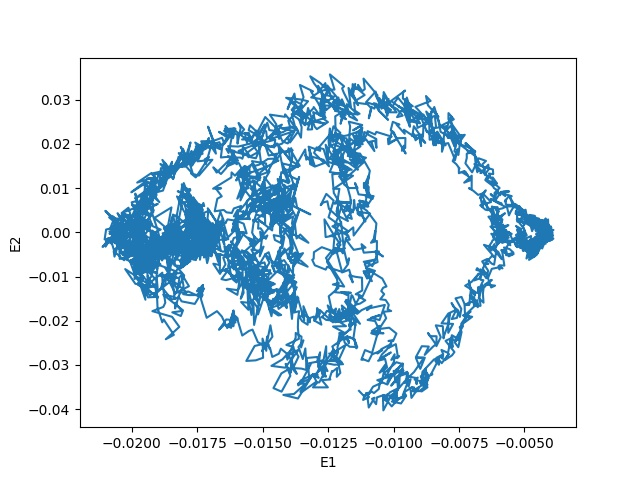
\includegraphics[width=\linewidth]{lamda_svd.jpg}
  \caption{Plot of E1 Vs E2 (top two right singular vectors) of data matrix for  timeseries $\lambda$ (non-stochastic) of \textit{GRS 1915 + 105}.}
  \label{lamda_svd}
\end{figure}


\section{Conclusion}
Exploring different techniques in order to have a conclusive inference for black hole systems turns out to be indispensable. We explore two different techniques for the first time in the literature to uncover  properties of black holes from the timeseries obtained from satellite data. Based on our analysis, we are able to identify two extreme temporal dynamical classes of accretion around black holes. We use Principal Component Analysis, a widely used technique to identify an prominent directionality in the data, in order to characterize the timeseries as Stochastic vs Non-stochastic. We further extend the Correlation Integral based studies by performing Singular Value Decomposition on the data matrix and using the right singular vectors in order to study temporal dynamics. Our results  are matching with previous Correlation Integral based studies in most of the cases.
% conference papers do not normally have an appendix


\begin{thebibliography}{1}
\bibitem{Mukhopadhyay2004}
 Mukhopadhyay, Banibrata. "Chaotic behavior of micro quasar GRS 1915+ 105." AIP Conference Proceedings. Vol. 714. No. 1. American Institute of Physics, 2004.

\bibitem{misra2006}
Misra, Ranjeev, et al. "The nonlinear behavior of the black hole system grs 1915+ 105." The Astrophysical Journal 643.2 (2006): 1114.

\bibitem{Bandt2002}
Bandt, Christoph, and Bernd Pompe. "Permutation entropy: a natural complexity measure for time series." Physical review letters 88.17 (2002): 174102.

\bibitem{Boaretto2021}
Boaretto, B. R. R., et al. "Discriminating chaotic and stochastic time series using permutation entropy and artificial neural networks." Scientific reports 11.1 (2021): 1-10.

\bibitem{lacasa2010}
  Lacasa, Lucas, and Raul Toral. "Description of stochastic and chaotic series using visibility graphs." Physical Review E 82.3 (2010): 036120.

\bibitem{Brunton2016}
  Brunton, Steven L., Joshua L. Proctor, and J. Nathan Kutz. "Discovering governing equations from data by sparse identification of nonlinear dynamical systems." Proceedings of the national academy of sciences 113.15 (2016): 3932-3937.

\bibitem{Adegoke2018}
Adegoke, Oluwashina, et al. "Correlating non-linear properties with spectral states of RXTE data: possible observational evidences for four different accretion modes around compact objects." Monthly Notices of the Royal Astronomical Society 476.2 (2018): 1581-1595.

\bibitem{Shakura1973}
Shakura, Ni I., and Rashid Alievich Sunyaev. "Black holes in binary systems. Observational appearance." Astronomy and Astrophysics 24 (1973): 337-355.

\bibitem{narayan1994}
  Narayan, Ramesh, and Insu Yi. "Advection-dominated accretion: Underfed black holes and neutron stars." arXiv preprint astro-ph/9411059 (1994).

  \bibitem{chakrabarti1995}
Chakrabarti, Sandip K., and Lev G. Titarchuk. "Spectral properties of accretion disks around galactic and extragalactic black holes." arXiv preprint astro-ph/9510005 (1995).

\end{thebibliography}

%https://heasarc.gsfc.nasa.gov/docs/xte/XTE.html
%https://heasarc.gsfc.nasa.gov/docs/xte/xte_public.html



\end{document}
